\chapter{Các hệ thống và công nghệ liên quan}

\section{ReGreT}

\textbf{ReGreT} \cite{regret-reputation-system} là một mô hình đánh giá uy tín trong xã hội nhiều tác nhân (multi-agent society), được xây dựng nhằm mô phỏng cách con người hình thành và sử dụng danh tiếng trong các tương tác xã hội.
Mô hình đưa ra ba chiều chính (dimension) của uy tín: chiều cá nhân (individual), chiều xã hội (social), và chiều bản thể học (ontological).

\subsection{Chiều cá nhân}

Đây là mức độ cơ bản nhất của uy tín, dựa trên trải nghiệm trực tiếp giữa hai tác nhân. Khi hai tác nhân tương tác, mỗi bên ghi nhận \textit{kết quả} (outcomes) từ tương tác đó, bao gồm những gì đã được thỏa thuận và những gì thực sự xảy ra.
Dựa vào những kết quả này, mỗi tác nhân hình thành \textit{ấn tượng cá nhân} (impression), từ đó tính ra \textit{uy tín chủ quan} (subjective reputation), dựa trên tập hợp các ấn tượng mà tác nhân $a$ từng ghi nhận về $b$.
Bên cạnh đó, cũng sẽ một
\textit{độ tin cậy} (reliability) đối với uy tín chủ quan này. Những ấn tượng gần thời điểm hiện tại hơn sẽ được ưu tiên cao hơn thông qua hàm trọng số thời gian.

Từ đó, ReGreT định nghĩa cách tính uy tín trực tiếp của một tác nhân $a$ đối với tác nhân $b$ theo chiều cá nhân như sau:
\[R_{a \rightarrow b}(subject)\]

\subsection{Chiều xã hội}

ReGreT mô hình hóa hiện tượng phổ biến trong xã hội con người: một cá nhân mang theo uy tín của nhóm mà họ thuộc về. Nếu không có đủ thông tin trực tiếp, ta có thể dựa vào uy tín nhóm để ước lượng hành vi của một tác nhân.
Tương tự như cách một cá nhân có thể bị ảnh hưởng bởi uy tín của nhóm mà mình thuộc về, bản thân cá nhân đó cũng sẽ dựa vào \textit{trải nghiệm} (experiences) của những người trong chính nhóm của mình để bổ sung và củng cố hiểu biết cá nhân về một thực thể.
Nói cách khác, những gì mà các thành viên trong nhóm từng trải qua với một thực thể cụ thể (hoặc với nhóm của thực thể đó) sẽ góp phần định hình và làm phong phú thêm nhận định của mỗi thành viên trong nhóm.

Do đó, để tính giá trị uy tín của mình đối với một tác nhân theo chiều xã hội, ReGreT mở rộng thêm ba nguồn thông tin mới. Bên cạnh tương tác trực tiếp với chính tác nhân, đồng thời cần xem xét thêm
tương tác với các thành viên trong nhóm mà tác nhân đó thuộc về, thông tin mà nhóm của mình đối với tác nhân đó, và cuối cùng là thông tin mà nhóm của mình đối với nhóm của tác nhân đó.

\subsubsection{Trải nghiệm cá nhân}

Giả sử ta tính giá trị uy tín của một tác nhân $a$ thuộc về nhóm $\mathcal{A}$ đối với tác nhân $b$ thuộc về nhóm $\mathcal{B}$.
Đầu tiên, ta đã biết uy tín trực tiếp giữa hai tác nhân như sau:
\[R_{a \rightarrow b}(subject)\]

Tiếp theo, sự tương tác của $a$ đối với các thành viên khác của nhóm $\mathcal{B}$ được biểu diễn như sau:
\[R_{a \rightarrow \mathcal{B}}(subject)=\sum_{b_i \in \mathcal{B}} \omega^{ab_i} \cdot R_{a \rightarrow b_i}(subject)\]
trong đó, $\displaystyle\sum_{b_i \in \mathcal{B}} \omega^{ab_i} = 1$.
Vì đang trong trường hợp uy tín chủ quan, chúng ta cần phương thức để thể thiện độ tin cậy của uy tín này:
\[RL_{a \rightarrow \mathcal{B}}(subject)=\sum_{b_i \in \mathcal{B}} \omega^{ab_i} \cdot RL_{a \rightarrow b_i}(subject)\]

\subsubsection{Trải nghiệm nhóm}

Một khi đã có được trải nghiệm của cá nhân $a$, ta sẽ xem xét đến trải nghiệm của nhóm $\mathcal{A}$ đối với tác nhân $b$ và cả nhóm $\mathcal{B}$.

Đầu tiên, ta tính uy tín chủ quan của nhóm $\mathcal{A}$ đối với tác nhân $b$ cùng với độ tin cậy của uy tín như sau:
\[R_{\mathcal{A} \rightarrow b}(subject)=\sum_{a_i \in \mathcal{A}} \omega^{a_ib} \cdot R_{a_i \rightarrow b}(subject)\]
\[RL_{\mathcal{A} \rightarrow b}(subject)=\sum_{a_i \in \mathcal{A}} \omega^{a_ib} \cdot RL_{a_i \rightarrow b}(subject)\]
trong đó, $\displaystyle\sum_{a_i \in \mathcal{A}} \omega^{a_ib} = 1$.

Tương tự, để biết được uy tín của nhóm $\mathcal{A}$ đối với nhóm $\mathcal{B}$, ta tính như sau:
\[R_{\mathcal{A} \rightarrow \mathcal{B}}(subject)=\sum_{a_i \in \mathcal{A}} \omega^{a_i\mathcal{B}} \cdot R_{a_i \rightarrow \mathcal{B}}(subject)\]
\[RL_{\mathcal{A} \rightarrow \mathcal{B}}(subject)=\sum_{a_i \in \mathcal{A}} \omega^{a_i\mathcal{B}} \cdot RL_{a_i \rightarrow \mathcal{B}}(subject)\]
trong đó, $\displaystyle\sum_{a_i \in \mathcal{A}} \omega^{a_i\mathcal{B}} = 1$.

\subsubsection{Tổng hợp tất cả thông tin lại với nhau}

Cuối cùng, ReGreT định nghĩa cách tính uy tín của tác nhân $a$ đối với tác nhân $b$ theo chiều xã hội như sau:
\begin{align*}
  SR_{a \rightarrow b}(subject) =\  & \xi_{ab} \cdot R_{a \rightarrow b}(subject) +                                       \\
                                    & \xi_{a\mathcal{B}} \cdot R_{a \rightarrow \mathcal{B}}(subject) +                   \\
                                    & \xi_{\mathcal{A}b} \cdot R_{\mathcal{A} \rightarrow b}(subject) +                   \\
                                    & \xi_{\mathcal{A}\mathcal{B}} \cdot R_{\mathcal{A} \rightarrow \mathcal{B}}(subject)
\end{align*}
\begin{align*}
  SRL_{a \rightarrow b}(subject) =\  & \xi_{ab} \cdot RL_{a \rightarrow b}(subject) +                                       \\
                                     & \xi_{a\mathcal{B}} \cdot RL_{a \rightarrow \mathcal{B}}(subject) +                   \\
                                     & \xi_{\mathcal{A}b} \cdot RL_{\mathcal{A} \rightarrow b}(subject) +                   \\
                                     & \xi_{\mathcal{A}\mathcal{B}} \cdot RL_{\mathcal{A} \rightarrow \mathcal{B}}(subject)
\end{align*}
trong đó, $\xi_{ab} + \xi_{a\mathcal{B}} + \xi_{\mathcal{A}b} + \xi_{\mathcal{A}\mathcal{B}} = 1$.

\subsection{Chiều bản thể học}

Trong hai chiều cá nhân và xã hội, mỗi lần đánh giá uy tín chỉ tập trung vào một khía cạnh đơn lẻ. Tuy nhiên, trong thực tế,
các khía cạnh này thường liên quan đến nhau và cần được kết hợp cùng \textit{trọng số} của từng khía cạnh lại để hình thành một khái niệm uy tín phức tạp hơn --
đó chính là mục tiêu của \textbf{chiều bản thể học}.

Ở chiều này, mô hình ReGreT sử dụng cấu trúc đồ thị để mô tả mối quan hệ giữa các khía cạnh khác nhau của uy tín.
Ví dụ, \textit{một người bán hàng tốt} (good seller) có thể bao gồm các yếu tố: giao hàng nhanh, giá cả hợp lý, và chất lượng sản phẩm cao,
ta có cấu trúc đồ thị bản thể như hình \ref{fig:good-seller-ontological-structure} để mô hình hóa mối quan hệ giữa các khía cạnh trong ví dụ này.

\begin{figure}[H]
  \centering
  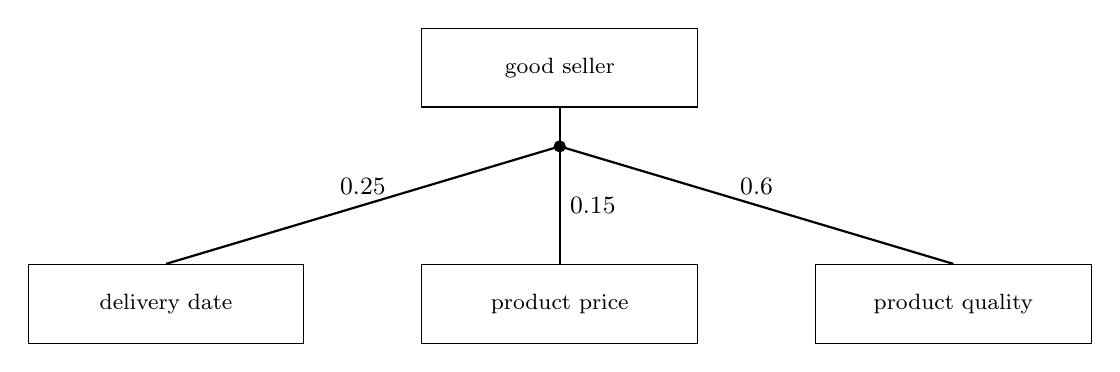
\begin{tikzpicture}
    \node[draw, rectangle, minimum width=3.5cm, minimum height=1cm, font=\footnotesize] at (5,0) (goodseller) {good seller};
    \node[draw, rectangle, minimum width=3.5cm, minimum height=1cm, font=\footnotesize] at (0,-3) (deliverydate) {delivery date};
    \node[draw, rectangle, minimum width=3.5cm, minimum height=1cm, font=\footnotesize] at (5,-3) (productprize) {product price};
    \node[draw, rectangle, minimum width=3.5cm, minimum height=1cm, font=\footnotesize] at (10,-3) (productquality) {product quality};

    \filldraw[black] (5,-1) circle (2pt);

    \draw[thick] (goodseller.south) -- (5,-1);
    \draw[thick, font=\small] (deliverydate.north) -- (5,-1) node[midway, above] {0.25};
    \draw[thick, font=\small] (productprize.north) -- (5,-1) node[midway, right] {0.15};
    \draw[thick, font=\small] (productquality.north) -- (5,-1) node[midway, above] {0.6};
  \end{tikzpicture}
  \caption{Cấu trúc đồ thị bản thể cho ``một người bán hàng tốt''}
  \label{fig:good-seller-ontological-structure}
\end{figure}

Vì vậy, khi muốn tính một uy tín phức hợp theo chiều bản thể học, một tác nhân cần tính uy tín của từng khía cạnh liên quan.
Mỗi khía cạnh này có thể lại là một nút trong một đồ thị con, nơi nó cũng được cấu thành từ các khía cạnh nhỏ hơn nữa.
Đây là một cấu trúc phân cấp đệ quy -- điểm rất đặc trưng của mô hình này.
Đối với những nút cuối cùng trong đồ thị (các khía cạnh cơ bản nhất của hành vi, gọi là \textit{atomic aspect}),
thì uy tín của chúng được tính dựa trên chiều cá nhân và chiều xã hội.

Sau khi có điểm uy tín cho từng nút con, điểm uy tín của một nút bất kỳ $i$ trong đồ thị bản thể sẽ được tính bằng cách kết hợp
các giá trị của các nút con của nó theo một công thức:
\[OR_{a \rightarrow b}(i) = \sum_{j \in children(i)} w_{ij} \cdot OR_{a \rightarrow b}(j)\]
\[ORL_{a \rightarrow b}(i) = \sum_{j \in children(i)} w_{ij} \cdot ORL_{a \rightarrow b}(j)\]
trong đó, $OR_{a \rightarrow b}(j) = SR_{a \rightarrow b}(j)$ khi $j$ là một khía cạnh cơ bản.

Đối với ví dụ ở hình \ref{fig:good-seller-ontological-structure}, ta có thể tính giá trị uy tín của $b$ (người bán hàng tốt)
theo góc nhìn của tác nhân $a$ bằng công thức:
\begin{align*}
  OR_{a \rightarrow b}(good\ seller) =\  & 0.25 \cdot SR_{a \rightarrow b}(delivery\ date) + \\
                                         & 0.15 \cdot SR_{a \rightarrow b}(product\ price) + \\
                                         & 0.6 \cdot SR_{a \rightarrow b}(product\ quality)
\end{align*}

\section{EigenTrust}

Mạng chia sẻ tập tin ngang hàng (P2P) đang ngày càng trở nên phổ biến nhờ ưu điểm không cần máy chủ trung tâm, có khả năng mở rộng tốt và cung cấp nhiều dữ liệu đa dạng.
Tuy nhiên, đặc tính ẩn danh và mở của P2P cũng khiến hệ thống này dễ bị lạm dụng, không ai chịu trách nhiệm rõ ràng cho nội dung mà họ chia sẻ. Kết quả là
tệp tin giả mạo, virus, hoặc nội dung bị chỉnh sửa có thể được phát tán rộng rãi, các peer độc hại có thể dễ dàng lừa người dùng tải về nội dung sai.
Trước những thách thức trên, một giải pháp hiệu quả là sử dụng cơ chế đánh giá danh tiếng giữa các peer trong mạng.

\textbf{EigenTrust} \cite{eigentrust-algorithm-for-reputation-management-in-2p2-networks} được giới thiệu là một thuật toán giảm thiểu khả năng tải về các tập tin độc hại
bằng cách gán mỗi peer một \textit{giá trị tin cậy toàn cục} (global trust value) duy nhất, dựa trên lịch sử tải lên của peer đó. Mỗi peer trong mạng cùng tham gia tính toán điểm tin cậy của nhau
theo cách phân tán và đối xứng. Khi tải tập tin về, các peer sẽ ưu tiên chọn nguồn tải là những peer có điểm tin cậy cao, giúp giảm đáng kể số lượng tập tin không xác thực.

\subsection{Giá trị tin cậy cục bộ}

Mỗi peer trong hệ thống mạng P2P cho phép theo dõi lịch sử giao dịch của nhau và đánh giá lẫn nhau sau mỗi giao dịch. Ví dụ, mỗi khi peer $i$ tải tập tin từ
peer $j$, nó có thể gán điểm tích cực $(tr(i, j) = 1)$ nếu hài lòng, hoặc điểm tiêu cực $(tr(i, j) = -1)$ nếu gặp vấn đề như tập tin bị hỏng, giả mạo hoặc quá trình tải thất bại.
Từ các đánh giá này, một \textit{giá trị tin cậy cục bộ} (local trust value) có thể được tính bằng cách cộng các điểm đánh giá mà peer $i$ đã gán cho $j$, biểu diễn là $s_{ij}=\sum tr_{ij}$.

Ngoài ra, có thể biểu diễn giá trị này bằng cách lưu số lượng giao dịch hài lòng $sat(i, j)$ và không hài lòng $unsat(i, j)$, rồi tính:
\[st_{ij} = sat(i, j) - unsat(i, j)\]

\subsubsection{Chuẩn hóa giá trị tin cậy cục bộ}

Trước tiên, cần chuẩn hóa các giá trị tin cậy cục bộ để đảm bảo tính công bằng. Nếu không chuẩn hóa, một peer độc hại có thể đánh giá tích cực cho các peer độc hại khác và
đánh giá tiêu cực cho các peer có uy tín cao. Để chuẩn hóa, ta chỉ xét các đánh giá tích cực, và tính xác suất chọn mỗi peer $j$ khi được peer $i$ tin tưởng như sau:
\[c_{ij} = \frac{max(s_{ij}, 0)}{\sum_{j} max(s_{ij}, 0)}\]
Cách làm này đảm bảo các giá trị $c_{ij}$ nằm trong khoảng $[0, 1]$ và có thể được hiểu như một xác suất trong mô hình ngẫu nhiên
(chú ý: nếu $\sum_{j} max(s_{ij}, 0) = 0$ thì $c_{ij}$ sẽ không xác định, vấn đề này sẽ được giải quyết sau đó).
Tuy nhiên, có một số hạn chế: nếu $c_{ij} = c_{ik}$ , ta chỉ biết mức độ tin tưởng của $i$ đối với $j$ và $k$ là như nhau, nhưng không rõ mức độ tuyệt đối đó là cao hay thấp.
Dù vậy, việc chuẩn hóa theo cách này giúp quá trình tính toán hiệu quả hơn và dễ dàng áp dụng mô hình xác suất.

\subsubsection{Tổng hợp các giá trị tin cậy cục bộ}

Sau khi chuẩn hóa, mục tiêu là tổng hợp các đánh giá cục bộ để thu được cái nhìn rộng hơn về độ tin cậy của từng peer.
Điều này được thực hiện bằng cách áp dụng \textbf{transitive trust} (tạm dịch: niềm tin chuyển tiếp)
-- nghĩa là peer $i$ sẽ hỏi ý kiến những người mà nó tin tưởng, và kết hợp đánh giá của họ với trọng số tương ứng.

Quá trình tổng hợp này dẫn đến một biểu thức dạng:
\[t_{ik} = \sum_{j} c_{ij}c_{jk}\]
trong đó, $t_{ik}$ thể hiện niềm tin của peer $i$ đối với $k$ sau khi hỏi bạn bè của nó $j$, mỗi người bạn của $i$ lại đánh giá $k$ một cách riêng $c_{jk}$.
Ta có thể biểu diễn biểu thức trên thành ma trận: nếu ta gọi $C$ là ma trận $[c_{ij}]$ và $\vec{t_i}$ là vector chứa các giá trị $t_{ik}$, khi đó ta có
$\vec{t_i} = C^{T}\vec{c_i}$.

Ý tưởng trên có thể được mở rộng bằng cách tiếp tục lan truyền niềm tin qua nhiều bước: từ bạn, đến bạn của bạn, đến bạn của bạn của bạn, v.v\dots
Điều này tương ứng với việc nâng ma trận lên lũy thừa: $(C^T)^2, (C^T)^3, ..., (C^T)^n$, và khi $n$ đủ lớn, vector $\vec{t_i}$ sẽ hội tụ về một vector
\textit{duy nhất cho mỗi peer} $i$ -- đó chính là vector riêng chính của ma trận tin cậy chuẩn hóa $C$. Nói cách khác, $\vec{t}$ là \textit{vector tin cậy toàn cục} (global trust vector) trong mô hình này,
và mỗi phần tử của nó, $\vec{t_j}$, định lượng mức độ tin cậy của hệ thống nói chung đặt vào peer $j$.

\subsection{Giải thích về xác suất}

Cách hiểu xác suất cung cấp một góc nhìn trực quan cho quá trình lan truyền uy tín trong mạng. Tưởng tượng có một tác nhân ngẫu nhiên đi lang thang trong mạng P2P
để tìm peer đáng tin. Tại mỗi bước, khi đang đứng ở peer $i$, nó sẽ chuyển đến peer $j$ với xác suất là $c_{ij}$ -- tức là mức độ mà $i$ tin tưởng $j$.
Quá trình này tạo thành một \textbf{xích Markov} \cite{markov-chain} với ma trận chuyển xác suất là ma trận tin cậy chuẩn hóa $C$.
Sau nhiều bước di chuyển, tác nhân sẽ thường xuyên rơi vào những peer đáng tin hơn -- và xác suất dừng lại ở mỗi peer chính là mức độ danh tiếng toàn cục.

Điều này giống như mô hình ``Random Surfer'' \cite{random-suffer-model-pagerank} trong PageRank: dù đi lung tung, người dùng sẽ thường ghé lại các trang web đáng tin và phổ biến hơn.
Cách hiểu xác suất này cung cấp một nền tảng trực quan và toán học để giải thích sự hội tụ về danh tiếng trong mạng.

\subsection{Triển khai EigenTrust}

\subsubsection{EigenTrust cơ bản}

Trong phiên bản đơn giản nhất, ta giả sử có một máy chủ trung tâm lưu trữ tất cả giá trị $c_{ij}$, mục tiêu chính là tính được giá trị tin cậy toàn cục
$\vec{t} = C^{T}\vec{e}$, với vector khởi đầu là $\vec{e}$ thể hiện phân bố xác suất đồng đều của toàn bộ $m$ peer, tức $e_i = 1/m$.
Chi tiết tại thuật toán \ref{alg:simple-eigentrust-algorithm}.

\begin{algorithm}
  \caption{Thuật toán EigenTrust đơn giản}
  \label{alg:simple-eigentrust-algorithm}
  \begin{algorithmic}
    \small
    \State $\vec{t}^{(0)} = \vec{e}$
    \Repeat
    \State $\vec{t}^{(k+1)} = C^{T}\vec{t}^{(k)}$
    \State $\delta = || \vec{t}^{(k+1)} - \vec{t}^{(k)} ||$
    \Until{$\delta < \epsilon$}
  \end{algorithmic}
\end{algorithm}

Tuy nhiên, có ba vấn đề thực tiễn mà thuật toán \ref{alg:simple-eigentrust-algorithm} không thể xử lý: nhóm peer có uy tín sẵn, những peer không hoạt động, và các peer độc hại hợp tác với nhau.

\textbf{Nhóm peer có uy tín sẵn.} Một hệ thống mạng P2P chỉ có một vài peer là có uy tín cao, thường là những người đầu tiên tham gia hệ thống, chẳng hạn như những nhà phát triển hay những người dùng truy cập sớm.
Ta định nghĩa tập hợp $P$ là các peer có uy tín sẵn (pre-trusted peers) và $\vec{p}$ là vector khởi đầu thay cho $\vec{e}$, với:
\[
  p_i =
  \begin{cases}
    1/|P| & ,\text{nếu } i \in P \\
    0     & ,\text{ngược lại}
  \end{cases}
\]
điều này giúp hội tụ nhanh hơn, cũng như loại bỏ được các peer độc hại.

\textbf{Những peer không hoạt động.} Nếu peer $i$ chưa từng tương tác với ai, thì không thể tính được $c_{ij}$.
Khi đó, ta mặc định rằng peer $i$ tin tưởng các peer uy tín sẵn theo phân phối $p$, tức $c_{ij} = p_j$. Ta có thể diễu diễn lại cách tính $c_{ij}$ như sau:
\[
  c_{ij} =
  \begin{cases}
    \frac{max(s_{ij}, 0)}{\sum_{j} max(s_{ij}, 0)} & , \text{nếu } \sum_{j} max(s_{ij}, 0) \neq 0 \\
    p_j                                            & , \text{ngược lại}
  \end{cases}
\]

\textbf{Các peer độc hại hợp tác với nhau.} Có khả năng sẽ xuất hiện nhiều nhóm peer độc hại mà chúng biết lẫn nhau, bọn chúng sẽ đánh giá cao lẫn nhau và đánh giá thấp những peer có uy tín.
Để ngăn chặn điều này, ta trộn thêm $\vec{p}$ vào mỗi vòng lặp:
\[\vec{t}^{(k+1)} = (1 - a)C^{T}\vec{t}^{(k)} + a\vec{p}\]
trong đó, $a$ là một hằng số nhỏ hơn 1. Việc này giúp ``kéo'' giá trị $\vec{c_i}$ của các peer về phía nhóm $P$ nhằm phá vòng lặp tin tưởng nội bộ của nhóm độc hại. Cuối cùng, ta hoàn thiện thuật toán EigenTrust cơ bản như sau:

\begin{algorithm}
  \caption{Thuật toán EigenTrust cơ bản}
  \label{alg:basic-eigentrust-algorithm}
  \begin{algorithmic}
    \small
    \State $\vec{t}^{(0)} = \vec{p}$
    \Repeat
    \State $\vec{t}^{(k+1)} = C^{T}\vec{t}^{(k)}$
    \State $\vec{t}^{(k+1)} = (1 - a)\vec{t}^{(k+1)} + a\vec{p}$
    \State $\delta = || \vec{t}^{(k+1)} - \vec{t}^{(k)} ||$
    \Until{$\delta < \epsilon$}
  \end{algorithmic}
\end{algorithm}

\subsubsection{EigenTrust phân tán}

Ở đây, bài toán được mở rộng để không cần máy chủ trung tâm, mà mỗi peer tự tính toán uy tín của chính mình bằng thông tin từ những peer từng tương tác với nó.
Yêu cầu đầu tiên của bài toán này là mỗi peer $i$ phải lưu trữ vector tin cậy cục bộ $\vec{c}_i$ và giá trị tin cậy toàn cục $t_i$ của chính nó.
Mỗi peer có thể tính giá trị tin cậy toàn cục của mình như sau:
\[t_i^{(k+1)} = (1 - a)(c_{1i}t_1^{(k)} + ... + c_{ni}t_n^{(k)}) + ap_i\]

Từ đó, ta có được thuật toán EigenTrust phân tán cơ bản được thể hiện ở thuật toán \ref{alg:distributed-eigentrust-algorithm}.
Vì mỗi peer chỉ tương tác với một số peer nhỏ (không phải toàn mạng), việc tính toán và truyền tin cũng nhẹ nhàng và hiệu quả.
Trong trường hợp một mạng lưới có nhiều peer hoạt động mạnh, ta có thể duy trì những lợi ích trên bằng cách giới hạn số lượng giá trị tin cậy cục bộ $c_{ij}$ mà mỗi peer
có thể báo cáo.

\begin{algorithm}
  \caption{Thuật toán EigenTrust phân tán}
  \label{alg:distributed-eigentrust-algorithm}
  \begin{algorithmic}
    \small
    \State $\textbf{Definitions}$
    \State \hspace{1em}- $A_i$: set of peers which have downloaded files from peer $i$
    \State \hspace{1em}- $B_i$: set of peers from which peer $i$ has downloaded files
    \State $\textbf{Algorithm}$
    \State Each peer $i$ do \{
    \State Query all peers $j \in A_i$ for $t_j^{0} = p_j$;
    \Repeat
    \State Compute $t_i^{(k+1)} = (1 - a)(c_{1i}t_1^{(k)} + c_{2i}t_2^{(k)} + ... + c_{ni}t_n^{(k)}) + ap_i$
    \State Send $c_{ij}t_i^{(k+1)}$ to all peers $j \in B_i$
    \State Compute $\delta = | t^{(k+1)} - t^{(k)} |$
    \State Wait for all peers of $j \in A_i$ to return $c_{ji}t_j^{(k+1)}$
    \Until{$\delta < \epsilon$}
    \State \}
  \end{algorithmic}
\end{algorithm}

\section{Slashdot}

\textbf{Slashdot} \cite{slashdot-web} là một trong những nền tảng cộng đồng trực tuyến đầu tiên, nổi bật với mô hình vận hành như một diễn đàn công cộng thực sự -- nơi người dùng không chỉ đọc tin tức mà còn có thể bình luận,
thảo luận và tranh luận về các chủ đề liên quan đến công nghệ, phần mềm mã nguồn mở, khoa học, và xã hội kỹ thuật số.
Điều làm nên sự đặc biệt của Slashdot không nằm ở bản thân nội dung, mà ở cách mà cộng đồng và hệ thống kỹ thuật cùng phối hợp để duy trì trật tự, chất lượng, và tính dân chủ của các cuộc đối thoại.

\subsection{Karma}

Trái tim của cơ chế tự điều chỉnh trên Slashdot là hệ thống \textbf{karma} \cite{mechanisms-of-website-slashdot} -- một công cụ định lượng uy tín và mức độ đóng góp của người dùng trong cộng đồng.
Karma không phải là một loại điểm số đơn thuần, mà là một dạng ``vốn xã hội kỹ thuật số''. Nó phản ánh việc người dùng có đưa ra những bình luận hữu ích, đóng góp xây dựng hay không.

Người dùng sẽ tăng karma nếu bình luận của họ được đánh giá cao bởi những người kiểm duyệt tạm thời (moderators); hoặc nội dung họ cung cấp có chất lượng, mang lại thông tin mới, sâu sắc hoặc hữu ích.
Ngược lại karma giảm đi khi người dùng đăng bình luận gây tranh cãi, xúc phạm, thiếu nội dung hoặc không liên quan; hoặc bị nhiều người đánh giá tiêu cực hoặc báo cáo vì hành vi không phù hợp.

Điểm karma không được hiển thị công khai dưới dạng con số cụ thể, nhưng nó tác động rõ rệt đến trải nghiệm và quyền hạn của người dùng:
\begin{itemize}
  \item Mức karma cao: người dùng có thể được lựa chọn làm moderator, có ảnh hưởng xã hội cao, bình luận thường được ưu tiên hiển thị.
  \item Mức karma trung bình: người dùng có thể tham gia thảo luận, gửi bình luận, tương tác bình thường.
  \item Mức karma thấp: bình luận của người dùng có thể bị ẩn, quyền đăng bài hoặc đánh giá bị giới hạn.
\end{itemize}

\subsection{Cơ chế kiểm duyệt do cộng đồng đảm nhiệm}

Người dùng có karma cao sẽ được chọn ngẫu nhiên làm moderator trong một khoảng thời gian ngắn. Vai trò của họ là:
\begin{itemize}
  \item Đọc các bình luận mới trên bài viết
  \item Đánh giá chất lượng mỗi bình luận bằng một thang điểm (thường từ -1 đến +5)
  \item Gắn nhãn cho bình luận như: Insightful (sâu sắc), Offtopic (lạc đề), Funny (vui nhộn), Troll (gây rối), v.v.
\end{itemize}

Đặc biệt, người được trao quyền kiểm duyệt không phải quản trị viên cố định, mà luôn là người dùng bình thường được hệ thống chọn dựa trên mức karma --
điều này tạo nên một cơ chế kiểm duyệt dân chủ và linh hoạt.

\subsection{Cơ chế đánh giá lại kiểm duyệt}

Để đảm bảo tính công bằng và hạn chế việc lạm quyền từ các moderator, Slashdot triển khai cơ chế \textbf{meta-moderation} -- tức là kiểm duyệt các hành động kiểm duyệt.
Người dùng có mức karma đủ cao có thể được chọn để đánh giá lại các hành động kiểm duyệt trước đó, cụ thể là:
\begin{itemize}
  \item Xem lại các bình luận đã được chấm điểm và gắn nhãn bởi một moderator khác (ẩn danh)
  \item Đưa ra nhận định về việc hành động kiểm duyệt đó có công bằng, chính xác hay không
\end{itemize}

Hệ thống từ đó điều chỉnh lại mức độ tin cậy của các moderator trong tương lai. Những người thường xuyên kiểm duyệt thiếu công bằng, gắn nhãn sai hoặc thiên vị sẽ ít có khả năng được chọn làm moderator sau này.

Cơ chế meta-moderation là một điểm độc đáo giúp Slashdot duy trì môi trường thảo luận dân chủ nhưng vẫn hiệu quả, nhờ vào sự giám sát chéo giữa các thành viên trong cộng đồng.

\subsection{Phối hợp giữa cộng đồng và kỹ thuật}

Cơ chế karma và moderation của Slashdot là sự phối hợp giữa hai yếu tố kỹ thuật và xã hội:
\begin{itemize}
  \item Về mặt kỹ thuật, hệ thống được thiết kế để tự động chọn moderator, xử lý hiển thị bình luận theo điểm đánh giá, và giới hạn quyền của người dùng có karma thấp.
  \item Về mặt xã hội, người dùng tự điều chỉnh hành vi của mình thông qua phần thưởng và hình phạt từ cộng đồng -- dưới dạng điểm karma. Điều này không chỉ giảm thiểu gánh nặng cho quản trị hệ thống mà còn tăng cường sự tham gia và tinh thần trách nhiệm của người dùng trong việc gìn giữ môi trường thảo luận lành mạnh.
\end{itemize}
